% Reducing Reflex Laboratory Testing Through CBC-Based Prediction of Diabetes-Range HbA1c
%From Routine Blood Counts to Targeted Glycemic Testing: An Exploratory NHANES Study
%Can Routine Blood Counts Improve Glycemic Screening? A Predictive Modeling Study Using NHANES

\documentclass[conference]{IEEEtran}
\usepackage[T1]{fontenc}
\usepackage[utf8]{inputenc}
\usepackage{cite}
\usepackage{graphicx}
\usepackage{float}
\usepackage{booktabs}
\usepackage{microtype}
\usepackage{xurl}
\usepackage[hidelinks]{hyperref}
\pdfstringdefDisableCommands{\def\sim{~}}
\urlstyle{same}
\Urlmuskip=0mu plus 2mu\relax
\newcommand{\doi}[1]{\href{https://doi.org/#1}{\nolinkurl{#1}}}
\newcommand{\pendingcite}[1]{#1}
\emergencystretch=1.5em

\title{Can Routine Blood Counts Improve Glycemic Screening? A Predictive Modeling Study Using NHANES}

\author{
\IEEEauthorblockN{Hamid Saeed\textsuperscript{1}, Setayesh Afshar\textsuperscript{1}, Jacob Kraft\textsuperscript{1}, Emmanuella Osifo\textsuperscript{1}, Ahenkan Yeboah\textsuperscript{1}}
\IEEEauthorblockA{\textsuperscript{1}Department of Biomedical Engineering, University of Calgary, Calgary, AB, Canada}
}

\begin{document}
\maketitle

\section{Introduction and Motivation}



Diabetes mellitus is a metabolic disorder characterized by persistently elevated blood glucose due to insufficient insulin production or action, and it can remain undiagnosed for years. Worldwide, an estimated 589 million adults aged 20--79 years were living with diabetes in 2024, and approximately four in ten were unaware of their condition \cite{idf2025}. In the United States, data from the August 2021--August 2023 cycle of the National Health and Nutrition Examination Survey (NHANES) show that slightly more than one in four adults aged 20 years and older with diabetes were undiagnosed \cite{gwira2024}, and most adults with prediabetes do not know they have it \cite{cdc2026}. Undiagnosed diabetes is most common among older adults and adults with obesity \cite{gwira2024}. Early diagnosis allows timely lifestyle changes and treatment, which can prevent or delay complications affecting eyes, kidneys, and cardiovascular system \cite{idf2025}.


Part of the problem is that detection depends on a clinician ordering an appropriate glycemic test, such as hemoglobin A1c (HbA1c) or fasting plasma glucose. By contrast, the complete blood count (CBC) is among the most frequently ordered laboratory tests \cite{horton2019}. Several CBC-derived indices, including red cell distribution width \cite{veeranna2012} and the neutrophil-to-lymphocyte ratio \cite{mertoglu2017}, have been associated with dysglycemia. These associations may reflect chronic low-grade inflammation and altered red blood cell turnover. If routinely collected CBC values carry predictive information, they could support a decision-support tool that interprets CBC results alongside demographic information to guide subsequent glycemic testing. Such a tool could prioritize testing for patients at high predicted risk and potentially reduce unnecessary testing for those at very low risk. Because a missed case leaves disease undetected while a false positive leads to additional testing and follow-up, such a tool must reliably identify true cases while limiting unnecessary investigation.


This project therefore asks: In U.S. adults without a prior diabetes diagnosis, does adding CBC indices to age and sex improve the prediction of dysglycemia, defined as an HbA1c of 5.7\% or higher (the prediabetes or diabetes range), in NHANES August 2021--August 2023?


NHANES provides CBC, HbA1c, demographic, and self-reported diagnosis data for the same participants, making the project feasible within the term. We will compare models using age and sex alone with models that also include CBC measurements, then evaluate their predictions on participants whose data were not used for training. The expected contribution is an estimate of how much CBC information improves these predictions, with emphasis on identifying true cases while limiting unnecessary follow-up, together with an openly shared, reproducible analysis pipeline. These findings could inform a proposed testing pathway, but demonstrating clinical benefit would require further validation.


\section{Background and Research Gap}

Diabetes assessment combines clinical risk factors with measurements of glycemic status. Demographic and clinical information helps identify individuals who warrant investigation, while HbA1c, fasting plasma glucose, and oral glucose tolerance testing provide evidence of abnormal glucose regulation. Bang et al.\cite{bang2009} developed a diabetes risk score using NHANES data and validated it in subsequent NHANES and external community cohorts. The score incorporated age, sex, family history, hypertension, obesity, and physical activity , demonstrating that routinely available information can support screening decisions.


Liu et al. \cite{liu2025} used NHANES demographic, anthropometric, behavioral, and health information to compare automated machine learning with logistic regression, support vector machines, random forest, and extreme gradient boosting . Their automated model achieved an AUROC of 0.909, with 70.3\% sensitivity and 92.6\% NPV \cite{liu2025}. However, its broad predictor set does not isolate whether adding CBC measurements improves prediction compared with using age and sex alone. It also used earlier NHANES data, adults with no prior diabetes, and a combined HbA1c/glucose/OGTT endpoint, so it is not a strict benchmark for our numbers \cite{liu2025}. A symptom-and-demographics model without laboratory measurements reported 99.36\% accuracy \cite{rahman2023}, high enough to warrant caution about evaluation artifacts. Accurately distinguishing individuals with and without diabetes does not establish whether a model helps clinicians select appropriate follow-up tests.


The biological rationale for CBC includes relationships between blood-cell characteristics, inflammation, and insulin resistance. Gkrania-Klotsas et al.\cite{gkrania2010} reported associations between higher white-cell counts and type 2 diabetes across cross-sectional and prospective studies, while identifying concerns about confounding and publication bias. Their 20-study meta-analysis reported RR 1.61 (95\% CI 1.45--1.79), though publication bias likely inflates this association \cite{gkrania2010}. White blood cell count also predicted incident diabetes in a 10-year Korean cohort of non-obese adults (HR 1.55, 95\% CI 1.10--2.18, n=4,211) \cite{park2021}. In the 866-person prospective Insulin Resistance Atherosclerosis Study, other white-cell associations weakened after full adjustment, while lymphocyte count remained significant (OR 1.96, 95\% CI 1.13--3.37), partly explained by insulin sensitivity \cite{lorenzo2014}. Neutrophil-to-lymphocyte ratio was not associated with incident diabetes \cite{lorenzo2014}, although it was higher in prediabetes and diabetes in a separate study; platelet-to-lymphocyte ratio showed a more complex pattern \cite{mertoglu2017}.


A 2026 study from Shenzhen University General Hospital investigated CBC-based prediction by comparing logistic regression, LightGBM, and neural-network models using CBC measurements, derived inflammatory ratios, age, sex, and BMI \cite{guo2026}. Its model achieved an AUROC of 0.791 in a separate patient group \cite{guo2026}. However, the study used data from a single hospital and defined its outcome as HbA1c \(\geq\)5.7\%, combining prediabetes-range and diabetes-range results. Calibration differences and variation across participant subgroups further limited interpretation \cite{guo2026}. A similar study recruited 9,704 Iranian adults and reported 9,000 observations after preprocessing; its bootstrap-forest model worked best, with age and WBC the strongest predictors \cite{mansoori2023}. A related 2026 study, using RBC, WBC, RDW, and clinical predictors like BMI and metabolic syndrome, reported ROC-AUC 0.73 and, at a 0.20 threshold, 61.8\% sensitivity, 70.7\% specificity, and 88.9\% NPV for new-onset diabetes \cite{kamkar2026}. This is a close precedent for the sensitivity/NPV trade-off in Section 5, though it predicts new disease in people without diabetes at baseline, a narrower population than ours.


Individual CBC values show mixed support. RDW is positively associated with HbA1c in healthy adults \cite{veeranna2012}, and a separate cohort found the same association but also found that lower RDW, not higher, predicts incident diabetes \cite{engstrom2014}. A study of people already diagnosed with diabetes similarly found higher RDW linked to lower odds of poor glycemic control (OR 0.3, 95\% CI 0.2--0.7) \cite{yin2018}. Thus, higher RDW tracks with higher HbA1c at a point in time but does not consistently predict worse outcomes going forward. These findings support investigating CBC patterns but show why individual inflammatory markers should not automatically be treated as reliable diagnostic indicators.


Outcome interpretation presents an additional challenge. English et al.\cite{english2015} found that anemia and abnormalities of erythrocyte indices can affect HbA1c independently of glucose concentrations . A CBC-based model may therefore capture influences on the HbA1c measurement itself, alongside information about metabolic dysfunction. This distinction must be considered when interpreting predictions and connecting them to recommendations for further investigation. Reflex testing, where one cheap test decides whether a costlier second test is needed, shows feasibility promise \cite{mcdermott2023}. However, our evidence here is a preprint about a different test, ferritin \cite{mcdermott2023}, and a risk-score study \cite{bang2009}; neither establishes that deferring a test is clinically safe.


The proposed project will compare demographic-only and CBC-plus-demographic models using public NHANES data to estimate the added value of CBC and the sensitivity/NPV trade-off at several thresholds, with diabetes assessment as the initial application. The variety of measurements within a CBC also suggests potential applications to other conditions, although these would require separate investigation. Results will inform a proposed testing pathway grounded in clinical guidance, balancing missed cases against unnecessary follow-up. NHANES can establish predictive value, while improvements in clinical test selection would require subsequent validation.


\section{Dataset and Responsible Use}

This project uses public-use data from the National Health and Nutrition Examination Survey (NHANES), August 2021--August 2023 cycle, obtained from the Centers for Disease Control and Prevention's National Center for Health Statistics (CDC/NCHS) and accessed on October 15, 2026. NHANES is a cross-sectional survey using a complex, multistage probability sample of the U.S. civilian, noninstitutionalized population. Its design, field operations, and cycle-specific analytical guidance are documented by Terry et al. \cite{terry2024} and NCHS \cite{nhanes_overview}. NHANES is suitable for this project because it provides linked CBC, demographic, and glycemic measurements for the same participants, enabling evaluation of whether routinely available CBC information can help identify participants likely to have abnormal glycemic results \cite{demo_l,cbc_l,ghb_l,glu_l,diq_l}.


The demographic (DEMO\_L), complete blood count (CBC\_L), glycohemoglobin (GHB\_L), fasting-glucose (GLU\_L), and diabetes-questionnaire (DIQ\_L) files are linked through the participant identifier SEQN \cite{demo_l,cbc_l,ghb_l,glu_l,diq_l}. The cycle includes 11,933 interviewed participants, of whom 8,860 completed examinations \cite{terry2024}. HbA1c and fasting-glucose components were eligible for examined participants aged 12 years or older \cite{ghb_l,glu_l}. One analytical case represents one participant; dependence arising from clustered sampling must be addressed through the survey design.


Candidate predictors include age, sex, white and red blood cell counts, hemoglobin, hematocrit, mean corpuscular volume, mean corpuscular hemoglobin, mean corpuscular hemoglobin concentration, red cell distribution width, platelet count, mean platelet volume, and five leukocyte differential percentages. Race/ethnicity, education, and income are also retained for descriptive analyses \cite{demo_l,cbc_l}. Candidate laboratory outcomes are fasting plasma glucose and HbA1c, assessed separately. Diabetes-range thresholds are \(\geq\)126 mg/dL and \(\geq\)6.5\%, respectively; broader dysglycemia thresholds are \(\geq\)100 mg/dL and \(\geq\)5.7\% \cite{ada_diagnosis}. DIQ010 records self-reported diabetes diagnosis \cite{diq_l}. The primary endpoint, age restrictions, and handling of previously diagnosed diabetes will be prespecified before modeling. Laboratory thresholds indicate screening categories rather than confirmed clinical diagnoses \cite{ada_diagnosis}.


Population-level analyses will use WTPH2YR for CBC/HbA1c and WTSAF2YR for fasting glucose, together with the stratum and primary sampling-unit variables SDMVSTRA and SDMVPSU \cite{nhanes_overview,cbc_l,ghb_l,glu_l}. Fasting eligibility and zero-weight records require explicit handling. Unavailable outcome measurements will not be classified as normal, and final sample sizes will be reported after eligibility and missing-data restrictions.


Public-use records omit identifying information. Under the NCHS Data User Agreement, the data will be used only for statistical reporting and analysis, without attempts to identify participants, reverse disclosure protections, or link records to individually identifiable datasets \cite{nchs_dua}. Sharing will be limited to public-use data, analysis code, and nonidentifying results. Detailed geographic information and exact interview or examination dates require separate Research Data Center approval \cite{rdc_nhanes}.


Representation limitations include survey nonresponse, blood-draw nonresponse, component eligibility, and differences between a community survey and clinical testing populations \cite{nhanes_overview}. Red-cell disorders can also affect HbA1c independently of glucose, complicating interpretation of CBC-based predictions \cite{ngsp_factors}. Evaluation will emphasize sensitivity and negative predictive value, uncertainty, and demographic subgroup performance. Because these cross-sectional files do not capture clinical ordering decisions, local test prices, or consequences of withholding testing, they cannot independently establish the safety or cost-effectiveness of a skip/order policy. Results will therefore support exploratory risk-stratified testing research; clinical use would require external validation and separate economic evaluation.


\section{Proposed Methods and Evaluation}


\begin{figure*}[!t]
\centering
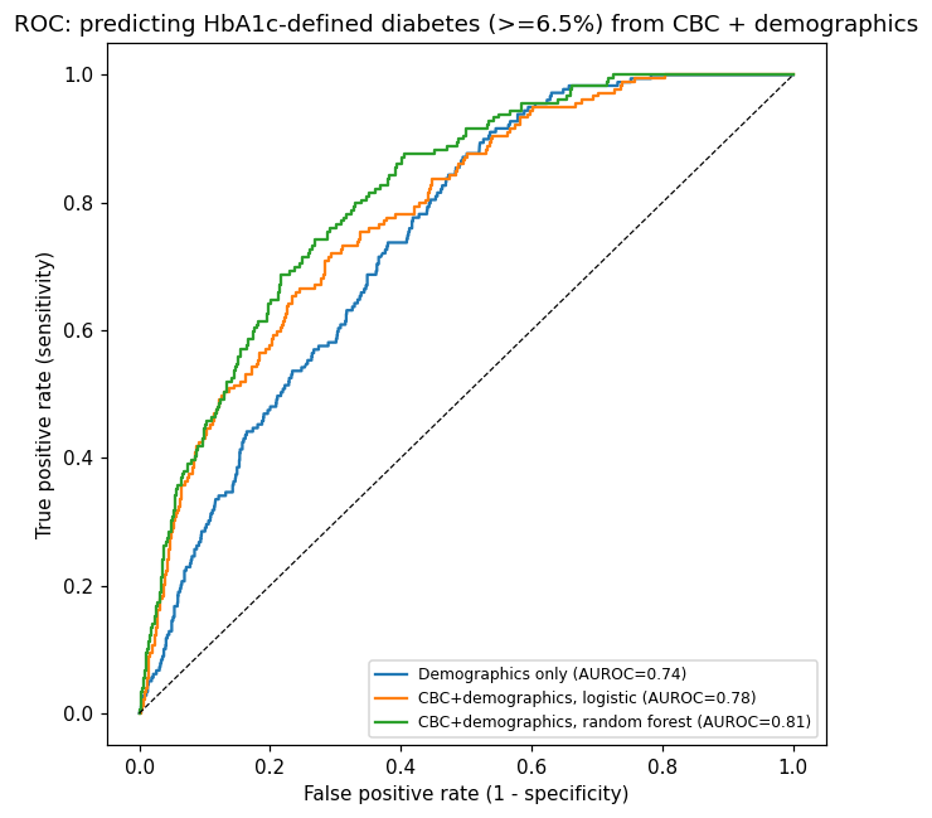
\includegraphics[width=0.76\textwidth]{roc_curves.png}
\caption{ROC curves on held-out test data: demographics only vs. two CBC+demographics models, predicting diabetes-range HbA1c.}
\label{fig:roc}
\end{figure*}

% Citations are linked to the bibliography entries used throughout the report.

\noindent\textbf{Study Design and Population:} This cross-sectional analysis uses data from the NHANES release covering August 2021 to August 2023. It aims to assess whether complete blood count (CBC) parameters can improve the identification of adults likely to have undiagnosed diabetes beyond what age and sex alone can determine. Predictors are CBC values (WBC and its breakdown, RBC, hemoglobin, hematocrit, MCV, RDW, platelet count) plus demographics (age, sex, race/ethnicity, education, income-to-poverty ratio) which will be combined using a participant sequence number (SEQN). Checks will be made for duplicate entries, unmatched records, missing data, and eligibility. We will finalize the intended population before the final report(e.g., adults only, no prior diagnosis); the current exploratory model includes participants as young as 12 and both diagnosed and undiagnosed cases. Exclusions include pregnant women, individuals with a prior diagnosis of diabetes, those currently using glucose-lowering medications, and those whose diabetes history cannot be clearly determined.


\noindent\textbf{Outcome and Predictors:} Our primary outcome is a diabetes-range HbA1c result (\(\geq\)6.5\%); we report eligible fasting glucose (\(\geq\)126 mg/dL) as a secondary check, since red-cell effects can bias HbA1c independent of true glycemic status \cite{english2015}. Self-reported diagnosis will define eligibility and stratify results, not serve as an interchangeable third outcome: in our data, 78.8\% of participants with a diabetes-range HbA1c already report a prior diagnosis, so a model built on this label currently distinguishes known from unknown cases more than it screens for new ones.The baseline model (Model 0) will include age and sex as predictors. The CBC-enhanced model (Model 1) will add WBC and its breakdown, RBC, hemoglobin, hematocrit, MCV, RDW, platelet count. Elastic-net logistic regression will be the primary method used.


\noindent\textbf{Cleaning and preprocessing:} We merge the five files by SEQN, starting from demographics and left-joining CBC, fasting glucose, HbA1c, and the questionnaire. Fasting glucose's subsample design makes missingness there structural, not an error. Each participant appears once. Race/ethnicity and education are currently passed to the models as raw numeric codes, which imposes an artificial ordering; we will fix this with proper categorical encoding, fit within each training fold, before the final report.


\noindent\textbf{Model Development and Survey Design:} We use Python (pandas, scikit-learn), comparing logistic regression, random forest, and gradient boosting, the same families used in \cite{guo2026}. A first working version runs end-to-end in \path{code/01_eda_cbc_glucose_demographics.ipynb} and \path{code/02_baseline_model_and_figures.ipynb} (Section 5), run from inside the \path{code/} directory, reproducible from the repository alone.


\noindent\textbf{Evaluation:} We judge models by sensitivity and NPV at several thresholds rather than a single accuracy or AUROC number, since missing a diagnosis matters more than an unnecessary test, similar in spirit to the operating-point approach in \cite{kamkar2026} and \cite{liu2025}. A first version is already in Section 5. We will report tests flagged and deferred together with the positive cases each threshold misses, rather than quoting NPV alone: a high NPV with low sensitivity mainly reflects how few participants are positive, not a safe deferral policy. Next, we will add stratified k-fold cross-validation with the pipeline refit per fold, design-aware confidence intervals, calibration checks, and a comparison against a simple age-only rule, before treating any threshold as a real recommendation. We will also compare the reduction in unnecessary glucose orders against an order-for-everyone baseline, following the reflex-testing framing in \cite{mcdermott2023}, while being clear this does not yet establish real-world cost or safety.


\noindent\textbf{Sensitivity, Reproducibility, and Limitations:} Sensitivity analyses will explore alternative outcomes related to blood sugar, the exclusion of individuals with prediabetes, restrictions to those without anemia, removal of certain red-cell indices, comparisons between weighted and unweighted models, and performance in subgroups by age and sex where feasible. The reporting will follow TRIPOD+AI guidelines. Limitations include the cross-sectional nature of the data, the use of a single measurement for outcome classification, the potential distortion of HbA1c readings due to red-cell biology, missing data, and the absence of external validation. Any promising model will be considered as a candidate for prioritizing confirmatory testing, rather than being used as a diagnostic tool.


\section{Preliminary Results}

Table 1 shows how many participants have each measurement in our merged NHANES 2021--2023 file (11,933 total). These are raw measurement counts, not yet restricted to each analysis's proper eligibility. For example, 311 of the 3,672 measured glucose results carry a zero fasting-sample weight and are not eligible for the fasting-glucose analysis, leaving about 3,361 eligible.



\begin{table}[H]
\caption{Measurement availability in the merged file.}
\label{tab:availability}
\centering
\footnotesize
\setlength{\tabcolsep}{3.6pt}
\renewcommand{\arraystretch}{1.18}
\begin{tabular}{@{}lrrr@{}}
\toprule
Measurement & \shortstack{n\\measured} & \shortstack{\% of\\merged file} & \shortstack{n with\\CBC too} \\
\midrule
CBC panel & 7,593 & 63.6\% & N/A \\
Fasting glucose & 3,672 & 30.8\% & 3,657 \\
HbA1c & 6,715 & 56.3\% & 6,689 \\
Self-reported diabetes & 11,736 & 98.3\% & 7,592 \\
\bottomrule
\end{tabular}
\end{table}

Two CBC values move the way Section 2 predicts: WBC and RDW both trend upward from normal to diabetes-range HbA1c status, though the difference is modest next to the spread within each group (full charts in notebook 01).


We fit three models on the subset with a complete CBC panel and HbA1c (n=6,678; 717, or 10.7\%, meet our HbA1c \(\geq\)6.5\% label, of whom 565, or 78.8\%, already report a prior diabetes diagnosis, so this model currently detects elevated HbA1c in a mixed diagnosed/undiagnosed group rather than screening for new cases). On a 75/25 split (5,008/1,670), test AUROC rose from 0.743 (demographics only) to 0.783 (logistic, with CBC) to 0.811 (random forest, with CBC). Figure 1 shows this as early evidence that CBC adds value beyond demographics in our own data.


% Figure 1 is queued above for two-column float placement.

The threshold matters more than any single summary number. At 0.10, the random forest flags 1,020 of 1,670 test participants, catching 94.4\% of positives but missing 10 of 179 (5.6\%). At 0.30, it flags 450, catching 68.7\% of positives but missing 56 of 179 (31.3\%), with 95.4\% NPV. That number sounds reassuring alone but still means roughly one in three true positives in the deferred group would be missed. A rule that always predicts "negative" would itself reach 89.3\% NPV with zero sensitivity, which is why NPV alone cannot show that deferral is safe.


\noindent\textbf{What we learned.} CBC-based signal measurably improves on demographics alone in our own data. This is encouraging for feasibility. It also surfaces real constraints: the cohort mixes known and unknown diabetes cases and includes minors; race and education are not yet properly encoded; and age dominates feature importance by a wide margin, with WBC, MCV, RDW, platelet, and RBC each adding only a little.


\noindent\textbf{Remaining limitations.} We have not applied survey weights or design variables (Section 3), validated with cross-validation or confidence intervals, checked calibration, restricted the cohort to an intended screening population, or compared against a simple age-only rule. All of this is planned before the final report (full list in the notebook's "Next steps").


\section{Teamwork and Project Plan }

Standing weekly roles:
\begin{itemize}
    \item Hamid Saeed: Project Manager
    \item Setayesh Afshar: Coordinator
    \item Jacob Kraft: Editor
    \item Ahenkan Yeboah: Reviewer
    \item Emmanuella Osifo: Presentation Lead
\end{itemize} 
\medskip

Milestones from this Research Plan through Dec. 4\textsuperscript{th}:
\begin{itemize}
    \item Oct 19\textsuperscript{th}–23\textsuperscript{rd} (stakeholder work ongoing since Oct 5\textsuperscript{th}): finalize the endpoint and cohort definition and apply survey weights; G. Assignment 3, led by Ahenkan Yeboah with Emmanuella Osifo.
    \item Oct 26\textsuperscript{th}–Nov 6\textsuperscript{th}: add cross-validation, calibration, and proper categorical encoding to the baseline models; G. Assignment 4, led by Hamid Saeed.
\item Nov 9\textsuperscript{th}–20\textsuperscript{th}: finish the sensitivity/NPV evaluation with confidence intervals; G. Assignment 5, led by Jacob Kraft.
\item Nov 23\textsuperscript{rd}–27\textsuperscript{th}: G. Assignment 6, Design Critique (lead TBD); turn the model into a draft policy.
\item Nov 30\textsuperscript{th}–Dec 4\textsuperscript{th}: Final Report and presentation, led by Emmanuella Osifo.
Every review pass follows our Team Contract: the lead adds evidence, Jacob Kraft checks clarity, Ahenkan Yeboah checks sources and methods, and everyone else reviews before submission.

\end{itemize}


\section*{Data and Code Availability}

Dataset: NHANES 2021--2023, CDC/NCHS, at \url{wwwn.cdc.gov/nchs/nhanes} (public, de-identified; no data use agreement needed; exact team access date to be confirmed).


GitHub repository: \url{https://github.com/hamidsaeed13/VORTEX-BMEN-600-Project}


\begin{itemize}
\item \path{README.md}: project overview, research question, and file map.
\item \path{code/01_eda_cbc_glucose_demographics.ipynb} and \path{code/02_baseline_model_and_figures.ipynb}: run from inside \path{code/} (they load data via a relative \path{../data/raw} path); produce every table and figure in this report.
\item Software: Python 3.9, pandas, numpy, matplotlib, scikit-learn.
\item Organized files: \path{data/raw/} (NHANES files + codebooks), \path{code/} (notebooks), \path{literature_review/} (source papers, with a README documenting what was checked against each one).
\end{itemize}


\section*{AI-Assisted Work}

Team members used AI tools, including Claude Code, ChatGPT, and Consensus, for literature search, drafting, data-analysis code, and troubleshooting, per our Team Contract's view of AI as a helper, not a replacement for our own judgment. Every AI-suggested journal source was checked against the publisher or an independent index, and every specific number in Section 2 was checked against that source's full text where available, across two independent review passes; \path{literature_review/README.md} lists exactly what was checked, what was corrected, and which sources we could only verify by title. The analysis code and its outputs were checked by rerunning them against the raw data; a human review of the full report and code by Ahenkan Yeboah, as Reviewer, is still to happen before submission.


\section*{Author Contributions}

\noindent\textbf{Hamid Saeed:} Defined the research question, gathered and merged the NHANES dataset,and built the preliminary baseline model wrote: Preliminary Results, Data and Code Availability section.\\
\noindent\textbf{Setayesh Afshar:} Conducted descriptive statistics on primary data analysis, basic and primary data pre-processing, wrote Dataset and Responsible Use, and merged different sections into on cohesive file. \\

\noindent\textbf{Emmanuella Osifo:} Conducted the literature review for the Introduction and motivation section.\\
\noindent\textbf{Jacob Kraft:} Constructed the background and research gap section, assessing possible limitations based on currently available research, and reviewed the introduction and proposed methods and evaluation. \\
\\
\noindent\textbf{Ahenkan Yeboah:} Authored the Proposed Methods and Evaluation section.


\begin{thebibliography}{30}

\bibitem{idf2025}
International Diabetes Federation, \emph{IDF Diabetes Atlas}, 11th ed. Brussels, Belgium: International Diabetes Federation, 2025. Accessed: Oct. 05, 2026. [Online]. Available: \url{https://diabetesatlas.org}

\bibitem{gwira2024}
J. Gwira, C. Fryar, and Q. Gu, ``Prevalence of total, diagnosed, and undiagnosed diabetes in adults: United States, August 2021--August 2023,'' National Center for Health Statistics, Hyattsville, MD, NCHS Data Brief 516, Nov. 2024, doi: \doi{10.15620/cdc/165794}.

\bibitem{cdc2026}
CDC, ``A U.S. Report Card,'' \emph{Diabetes}. Accessed: Oct. 05, 2026. [Online]. Available: \url{https://www.cdc.gov/diabetes/communication-resources/diabetes-statistics.html}

\bibitem{horton2019}
S. Horton \emph{et al.}, ``The Top 25 Laboratory Tests by Volume and Revenue in Five Different Countries,'' \emph{Am. J. Clin. Pathol.}, vol. 151, no. 5, pp. 446--451, Apr. 2019, doi: \doi{10.1093/ajcp/aqy165}.

\bibitem{veeranna2012}
V. Veeranna, S. K. Zalawadiya, S. S. Panaich, K. Ramesh, and L. Afonso, ``The Association of Red Cell Distribution Width with Glycated Hemoglobin among Healthy Adults without Diabetes Mellitus,'' \emph{Cardiology}, vol. 122, no. 2, pp. 129--132, 2012, doi: \doi{10.1159/000339225}.

\bibitem{mertoglu2017}
C. Mertoglu and M. Gunay, ``Neutrophil-Lymphocyte ratio and Platelet-Lymphocyte ratio as useful predictive markers of prediabetes and diabetes mellitus,'' \emph{Diabetes Metab. Syndr.}, vol. 11 Suppl 1, pp. S127--S131, Nov. 2017, doi: \doi{10.1016/j.dsx.2016.12.021}.

\bibitem{bang2009}
H. Bang \emph{et al.}, ``Development and validation of a patient self-assessment score for diabetes risk,'' \emph{Ann. Intern. Med.}, vol. 151, no. 11, pp. 775--783, Dec. 2009, doi: \doi{10.7326/0003-4819-151-11-200912010-00005}.

\bibitem{liu2025}
J. Liu, F. Ssewamala, R. An, and M. Ji, ``Use of automated machine learning to detect undiagnosed diabetes in US adults: Development and validation study,'' \emph{JMIR AI}, vol. 4, Art. no. e68260, Oct. 2025, doi: \doi{10.2196/68260}.

\bibitem{rahman2023}
M. A. Rahman, L. F. Abdulrazak, M. M. Ali, I. Mahmud, K. Ahmed, and F. M. Bui, ``Machine learning-based approach for predicting diabetes employing socio-demographic characteristics,'' \emph{Algorithms}, vol. 16, no. 11, Art. no. 503, 2023, doi: \doi{10.3390/a16110503}.

\bibitem{gkrania2010}
E. Gkrania-Klotsas \emph{et al.}, ``Differential white blood cell count and type 2 diabetes: Systematic review and meta-analysis of cross-sectional and prospective studies,'' \emph{PLoS ONE}, vol. 5, no. 10, Art. no. e13405, Oct. 2010, doi: \doi{10.1371/journal.pone.0013405}.

\bibitem{park2021}
J.-M. Park, H. S. Lee, J.-Y. Park, D.-H. Jung, and J.-W. Lee, ``White blood cell count as a predictor of incident type 2 diabetes mellitus among non-obese adults: A longitudinal 10-year analysis of the Korean Genome and Epidemiology Study,'' \emph{J. Inflamm. Res.}, vol. 14, pp. 1235--1242, Apr. 2021, doi: \doi{10.2147/JIR.S300026}.

\bibitem{lorenzo2014}
C. Lorenzo, A. J. Hanley, and S. M. Haffner, ``Differential white cell count and incident type 2 diabetes: The Insulin Resistance Atherosclerosis Study,'' \emph{Diabetologia}, vol. 57, no. 1, pp. 83--92, Jan. 2014, doi: \doi{10.1007/s00125-013-3080-0}.

\bibitem{guo2026}
X. Guo, N. Zhang, B. Li, X. Yu, J. Guo, and G. Dan, ``Using machine learning to identify individuals at elevated risk of diabetes from low-cost complete blood count data for opportunistic screening,'' \emph{Sci. Rep.}, vol. 16, Art. no. 29445, 2026, doi: \doi{10.1038/s41598-026-59213-3}.

\bibitem{mansoori2023}
A. Mansoori \emph{et al.}, ``Prediction of type 2 diabetes mellitus using hematological factors based on machine learning approaches: A cohort study analysis,'' \emph{Sci. Rep.}, vol. 13, Art. no. 663, 2023, doi: \doi{10.1038/s41598-022-27340-2}.

\bibitem{kamkar2026}
N. Kamkar \emph{et al.}, ``A machine learning-based framework for predicting type 2 diabetes mellitus using hematological indices,'' \emph{Am. Heart J. Plus}, vol. 69, Art. no. 100854, 2026, doi: \doi{10.1016/j.ahjo.2026.100854}.

\bibitem{engstrom2014}
G. Engstr\"om, J. G. Smith, M. Persson, P. M. Nilsson, O. Melander, and B. Hedblad, ``Red cell distribution width, haemoglobin A 1c and incidence of diabetes mellitus,'' \emph{J. Intern. Med.}, vol. 276, no. 2, pp. 174--183, Aug. 2014, doi: \doi{10.1111/joim.12188}.

\bibitem{yin2018}
Y. Yin, S. Ye, H. Wang, B. Li, A. Wang, W. Yan, J. Dou, and Y. Mu, ``Red blood cell distribution width and the risk of being in poor glycemic control among patients with established type 2 diabetes,'' \emph{Ther. Clin. Risk Manag.}, vol. 14, pp. 265--273, 2018, doi: \doi{10.2147/TCRM.S155753}.

\bibitem{english2015}
E. English, I. Idris, G. Smith, K. Dhatariya, E. S. Kilpatrick, and W. G. John, ``The effect of anaemia and abnormalities of erythrocyte indices on HbA1c analysis: A systematic review,'' \emph{Diabetologia}, vol. 58, no. 7, pp. 1409--1421, Jul. 2015, doi: \doi{10.1007/s00125-015-3599-3}.

\bibitem{mcdermott2023}
M. McDermott, A. Dighe, P. Szolovits, Y. Luo, and J. Baron, ``Using machine learning to develop smart reflex testing protocols,'' \emph{arXiv preprint arXiv:2302.00794}, Feb. 2023, doi: \doi{10.48550/arXiv.2302.00794}.

\bibitem{terry2024}
A. L. Terry, M. M. Chiappa, J. McAllister, D. A. Woodwell, and J. E. Graber, ``Plan and operations of the National Health and Nutrition Examination Survey, August 2021--August 2023,'' \emph{Vital Health Stat. 1}, no. 66, May 2024, doi: \doi{10.15620/cdc/151927}.

\bibitem{nhanes_overview}
National Center for Health Statistics, ``Brief overview of sample design, nonresponse bias assessment, and analytic guidelines for NHANES August 2021--August 2023,'' Sep. 2024. Accessed: Oct. 15, 2026. [Online]. Available: \url{https://wwwn.cdc.gov/nchs/nhanes/continuousnhanes/overviewbrief.aspx?Cycle=2021-2023}

\bibitem{demo_l}
National Center for Health Statistics, ``Demographic variables and sample weights (DEMO\_L): August 2021--August 2023 data documentation, codebook, and frequencies,'' Sep. 2024. Accessed: Oct. 15, 2026. [Online]. Available: \url{https://wwwn.cdc.gov/Nchs/Data/Nhanes/Public/2021/DataFiles/DEMO_L.htm}

\bibitem{cbc_l}
National Center for Health Statistics, ``Complete blood count with 5-part differential in whole blood (CBC\_L): August 2021--August 2023 data documentation, codebook, and frequencies,'' Sep. 2024. Accessed: Oct. 15, 2026. [Online]. Available: \url{https://wwwn.cdc.gov/Nchs/Data/Nhanes/Public/2021/DataFiles/CBC_L.htm}

\bibitem{ghb_l}
National Center for Health Statistics, ``Glycohemoglobin (GHB\_L): August 2021--August 2023 data documentation, codebook, and frequencies,'' Sep. 2024. Accessed: Oct. 15, 2026. [Online]. Available: \url{https://wwwn.cdc.gov/Nchs/Data/Nhanes/Public/2021/DataFiles/GHB_L.htm}

\bibitem{glu_l}
National Center for Health Statistics, ``Plasma fasting glucose (GLU\_L): August 2021--August 2023 data documentation, codebook, and frequencies,'' Sep. 2024. Accessed: Oct. 15, 2026. [Online]. Available: \url{https://wwwn.cdc.gov/Nchs/Data/Nhanes/Public/2021/DataFiles/GLU_L.htm}

\bibitem{diq_l}
National Center for Health Statistics, ``Diabetes (DIQ\_L): August 2021--August 2023 data documentation, codebook, and frequencies,'' Sep. 2024. Accessed: Oct. 15, 2026. [Online]. Available: \url{https://wwwn.cdc.gov/Nchs/Data/Nhanes/Public/2021/DataFiles/DIQ_L.htm}

\bibitem{ada_diagnosis}
American Diabetes Association, ``Diabetes diagnosis.'' Accessed: Oct. 15, 2026. [Online]. Available: \url{https://diabetes.org/about-diabetes/diagnosis}

\bibitem{nchs_dua}
National Center for Health Statistics, ``Data user agreement,'' Sep. 17, 2024. Accessed: Oct. 15, 2026. [Online]. Available: \url{https://www.cdc.gov/nchs/policy/data-user-agreement.html}

\bibitem{rdc_nhanes}
Centers for Disease Control and Prevention, Research Data Center, ``National Health and Nutrition Examination Survey,'' Nov. 20, 2024. Accessed: Oct. 15, 2026. [Online]. Available: \url{https://www.cdc.gov/rdc/restricted-nchs-variables/nhanes.html}

\bibitem{ngsp_factors}
NGSP, ``Factors that interfere with HbA1c test results,'' updated Jun. 23, 2026. Accessed: Oct. 15, 2026. [Online]. Available: \url{https://ngsp.org/factors.asp}

\end{thebibliography}


\end{document}